\newpage
\begin{appendices}
\section{Lexique}
\begin{itemize}
	\item EDT~:
	EDT est un acronyme signifiant Event Dispatch Thread. Concrètement, EDT est le thread principal s'occupant de la partie graphique d'une application Java, c'est-à-dire le dessin de l'IHM ou la gestion des interactions avec l'utilisateur.
	\newline

	\item Itérateur~:
	En programmation, un itérateur est un objet permettant de parcourir un tableau ou une collection, non pas nécessairement depuis le début du tableau, mais depuis n'importe quel index du tableau. Dans le cadre de notre projet, notre itérateur nous permet de parcourir notre Board.
	\newline

	\item Pair à pair~:
    Le pair à  pair (ou peer-to-peer en anglais), est un modèle de réseau permettant à deux machines de discuter d'égale à égale.
    Dans les faits, cela s'explique par le fait qu'une machine se connecte à une autre machine et inversement afin que celles-ci puissent s'échanger des informations sans passer par un serveur distant.
    \newline
    
   	\item Protocole réseau~:
    Un protocole est une méthode standard qui permet la communication entre des processus (s'exécutant éventuellement sur différentes machines), c'est-à-dire un ensemble de règles et de procédures à respecter pour émettre et recevoir des données sur un réseau. 
    Il en existe plusieurs selon ce que l'on attend de la communication. Certains protocoles seront par exemple spécialisés dans l'échange de fichiers (le FTP), d'autres pourront servir à gérer simplement l'état de la transmission et des erreurs (c'est le cas du protocole ICMP), ... 
	\newline

	\item Protocole TCP~: 
    Acronyme de Transmission Control Protocol, le protocole TCP/IP est le protocole standard utilisé sur internet, pour la liaison entre deux ordinateurs.
    Le protocole TCP vérifie la validité des paquets après leur réception afin d'être sûr de la validité de celle-ci.
    Le protocole TCP est située sur la couche 4 (couche de transport) du modèle OSI. 
	\newline
	
	\item Protocole UDP~:
    Acronyme User Datagram Protocol, le protocole UDP est un des protocoles standards utilisé sur internet. 
    La différence avec TCP est que les paquets sont reçus sous forme de datagrammes qui doivent être vérifiés pour valider la qualité du paquet reçu.
    Le protocole UDP est très utilisé, notamment, dans le cadre du jeu en ligne, ou encore le streaming, car la perte de paquet influe peu sur la quantité reçus.
    Le protocole UDP est située sur la couche 4 (couche de transport) du modèle OSI, au même titre que le protocole TCP. 
   \newline

	\item Socket~:
    Une socket est une interface de connexion bidirectionnelle permettant l'échange de données entre deux processus (distants ou non).
	\newline
 
	\item Socket de Berkeley~:
    Les sockets de Berkeley, sont un ensemble normalisés de fonctions de communications lancé par l'université de Berkeley au début des années 1980.
    De nos jours, elle est la norme utilisé par quasiment l'ensemble des langages de développement (C, Java, Python, ...).
    \newline
  
	\item Socket d'écoute~:
    Une socket d'écoute est une socket présente uniquement dans le protocole TCP. En effet, son rôle consiste, comme son nom l'indique, à écouter les demandes de connexion de socket externe sur un port prédéfini, afin de créer une socket qui permettra ensuite l'échange de données avant de reprendre son rôle d'écouteur.
	\newline
  
	\item Socket de service~:
    La socket de service est la socket crée par la socket d'écoute lorsque celle-ci reçoit une demande de connexion. La socket de service permet la communication entre le serveur et le client ayant fait une demande de connexion. C'est par cette socket que transitent toutes les données émises par le client et le serveur.
	\newline
  
	\item Thread~:
	Un thread est une sorte de processus, dit "léger". Le rôle d'un thread est d'exécuter une suite d'instruction précise que l'on peut nomme routine.
	Le fait de lancer une application informatique lance automatiquement un thread, celui-ci peut alors créer d'autres threads afin de délégué par exemple une tâche longue a un autre thread, afin que le thread principal (main thread), puisse continuer son fil d'exécution à lui.
	\newline

   
\end{itemize}


\newpage
\section{Webographie}
\begin{itemize}
	\item Fonctionnement des intelligences artificielles~: \url{http://www.datagenetics.com/blog/december32011/index.html}
\newline	
	\item API Java~: \url{https://docs.oracle.com/javase/7/docs/api/}
	\newline
	\item Règles de la bataille navale: \url{http://www.regles-de-jeux.com/regle-de-la-bataille-navale/}
\end{itemize}

\newpage
\section{Schéma du protocole de l'application}
\begin{sidewaysfigure}
    \centering
    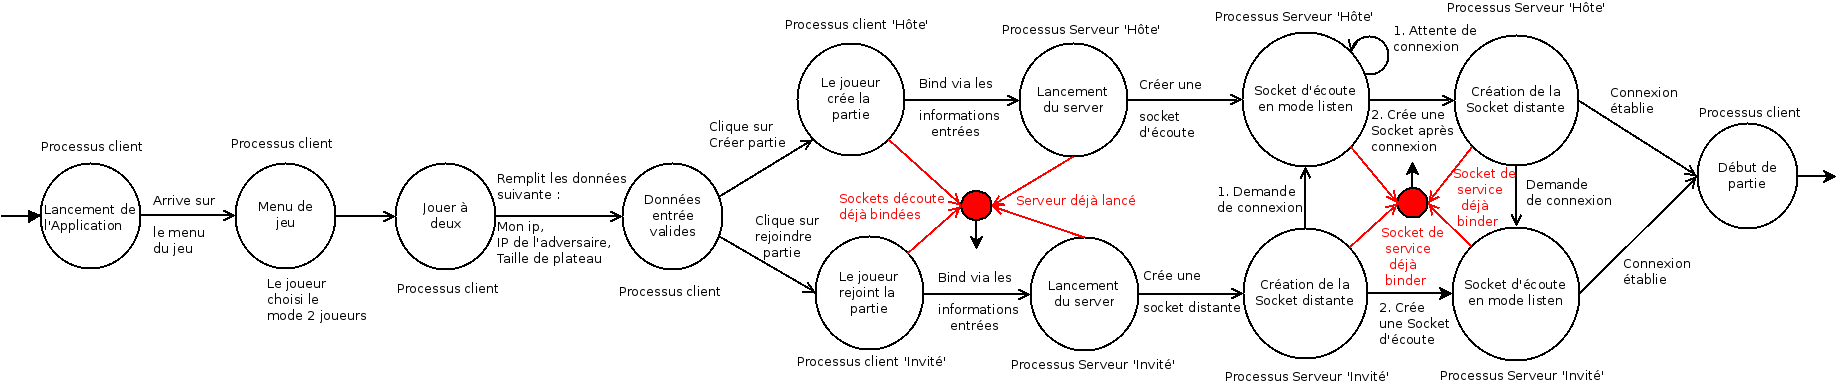
\includegraphics [width=215mm]{images/connection_between_players.png}
    \caption{Schéma représentant le protocole de connexion entre deux joueurs}
    \label{connection}
\end{sidewaysfigure}
\begin{sidewaysfigure}
    \centering
    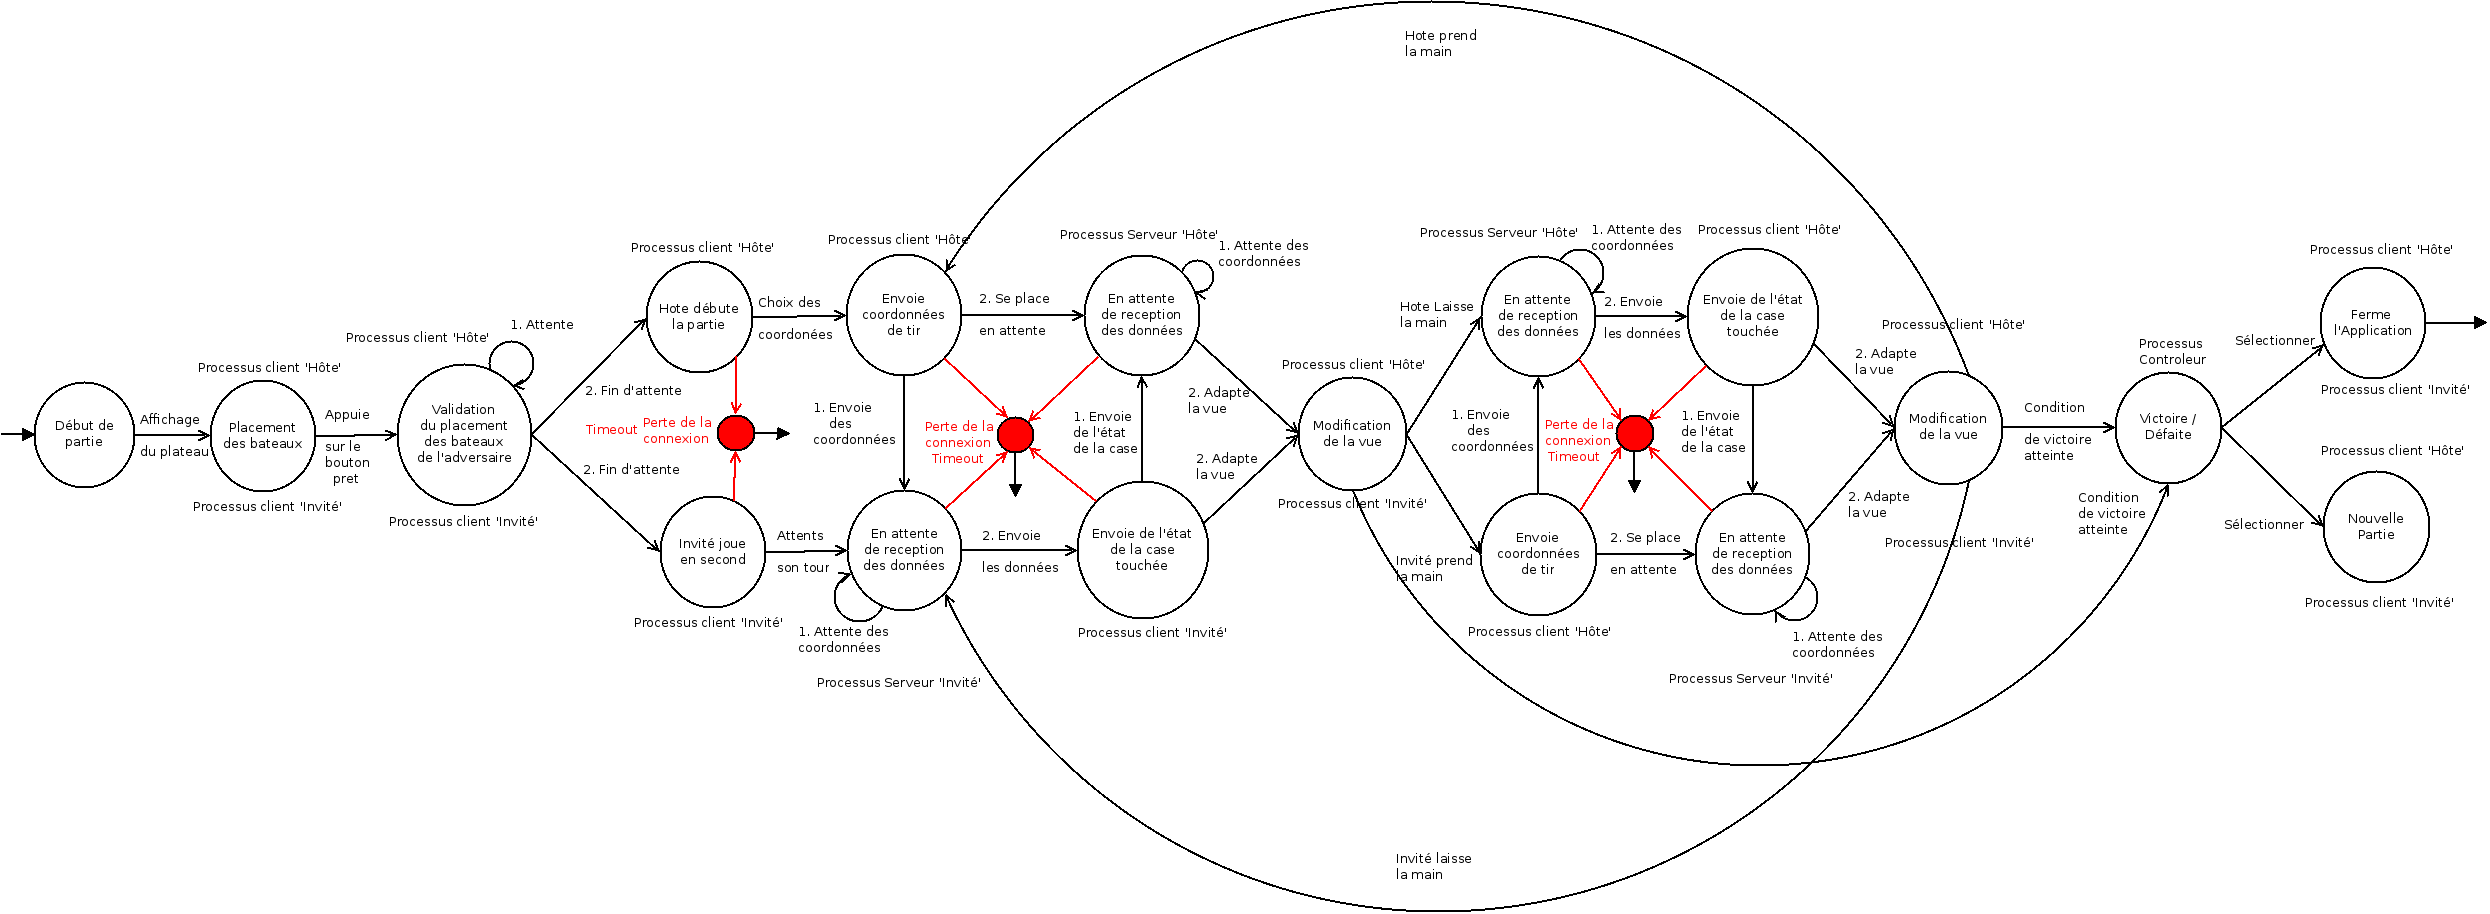
\includegraphics [width=215mm]{images/data_exhange_between_players.png}
    \caption{Schéma représentant le protocole d'échange de données entre deux joueurs}
    \label{connection}
\end{sidewaysfigure}

\end{appendices}
